\documentclass[varwidth=true, border=2pt]{standalone}
\usepackage{xcolor}
\usepackage{tikz}
\usetikzlibrary{trees}
\def\name#1{\hbox to 50pt{#1\rule{10pt}{0pt}}}
\begin{document}
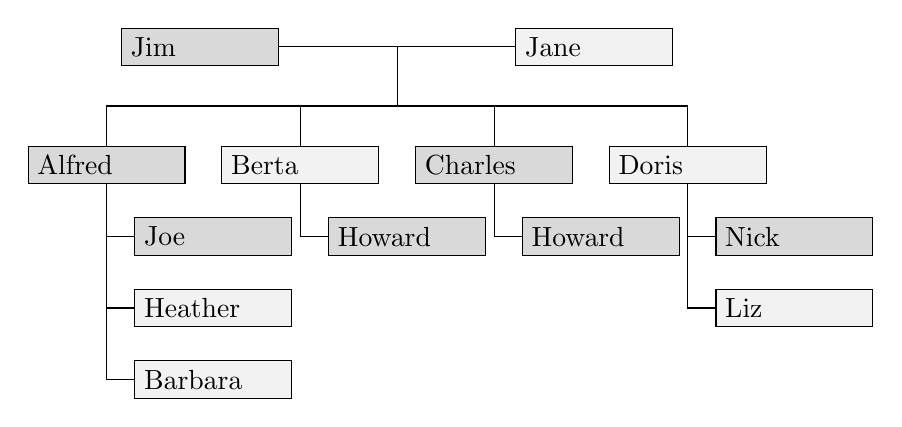
\begin{tikzpicture}[
  man/.style={rectangle,draw,fill=gray!30},
  woman/.style={rectangle,draw,fill=gray!10},
  grandchild/.style={grow=down,xshift=1em,anchor=west,
    edge from parent path={(\tikzparentnode.south) |- (\tikzchildnode.west)}},
  first/.style={level distance=6ex},
  second/.style={level distance=12ex},
  third/.style={level distance=18ex},
  level 1/.style={sibling distance=70pt}]
    % Parents
    \coordinate
      child[grow=left] {node[man,anchor=east]{\name{Jim}}}
      child[grow=right] {node[woman,anchor=west]{\name{Jane}}}
      child[grow=down,level distance=0ex]
    [edge from parent fork down]
    % Children and grandchildren
    child{node[man] {\name{Alfred}}
      child[grandchild,first] {node[man]{\name{Joe}}}
      child[grandchild,second] {node[woman]{\name{Heather}}}
      child[grandchild,third] {node[woman] {\name{Barbara}}}}
    child{node[woman] {\name{Berta}}
      child[grandchild,first] {node[man]{\name{Howard}}}}
    child {node[man] {\name{Charles}}
       child[grandchild,first] {node[man]{\name{Howard}}}}
    child {node[woman]{\name{Doris}}
      child[grandchild,first] {node[man]{\name{Nick}}}
      child[grandchild,second] {node[woman]{\name{Liz}}}};
\end{tikzpicture}
\end{document}
